% Appendix: Cold-Start vs Warmup Prior Regret

\section{Cold-Start vs Warmup Priors}
\label{sec:warmup_ablation}

Section~\ref{sec:warmup} introduces offline-to-online warmup priors,
which let the router begin with informed beliefs about each model's
strengths by loading sufficient statistics fitted on historical data.
Two natural questions arise when deciding whether to enable this
feature.

\paragraph{Q1: Do warmup priors reduce cold-start regret in practice?}
A practitioner choosing between enabling warmup priors or deploying
with a blank slate needs an apples-to-apples comparison where
\emph{each} condition uses its own best hyperparameters---the
configuration the practitioner would actually run.
We therefore compare ParetoBandit with warmup priors
($\alpha{=}\waAlpha$, $n_\mathit{eff}{=}\waNeff$,
$\gamma{=}\waGamma$) against Tabula Rasa
($\alpha{=}\waAlpha$, $n_\mathit{eff}{=}1$,
$\gamma{=}\waTRGamma$), each tuned independently via the
Pareto-knee procedure (Appendix~\ref{sec:hparam_sweep}).

\paragraph{Q2: Is the improvement actually from the priors, or from
a confounded hyperparameter?}
The ``best vs best'' comparison above has a subtle confound.
Because the Pareto-knee sweep selects different forgetting factors
for each condition ($\gamma{=}\waGamma$ for warmup vs.\
$\waTRGamma$ for Tabula Rasa), a skeptic could attribute the
improvement to the different memory lengths (${\sim}333$ vs.\
${\sim}250$ effective-memory steps) rather than to the priors
themselves.
To isolate the prior contribution, we add a \emph{matched-$\gamma$
control}: Tabula Rasa run at warmup's $\gamma{=}\waGamma$
(cold start, $n_\mathit{eff}{=}1$), so the only remaining
difference is prior strength.
All three conditions share $\alpha{=}\waAlpha$ and differ only in
prior strength ($n_\mathit{eff}{=}\waNeff$ for warmup vs.\ $1$
for both cold starts) and forgetting factor
($\gamma{=}\waGamma$ for warmup and the matched control vs.\
$\gamma{=}\waTRGamma$ for Tabula Rasa's independently optimised
configuration).

\medskip\noindent
Both questions are evaluated on the $K{=}3$ stationary portfolio
under four budget regimes: unconstrained (no pacer), tight
($B{=}\$3.0{\times}10^{-4}$/req), moderate
($B{=}\$6.6{\times}10^{-4}$/req), and loose
($B{=}\$1.87{\times}10^{-3}$/req).

\paragraph{Statistical methodology.}
We assess each comparison along two dimensions.
The first is \emph{typical-case} regret: does warmup
tend to outperform seed-by-seed?
The second is \emph{tail risk}: does warmup avoid
outlier runs where regret is disproportionately high?
We call a seed a \textbf{catastrophic failure} when its
cumulative regret exceeds $2{\times}$ the pooled median across
all conditions in that budget regime (warmup, Tabula Rasa,
and matched-$\gamma$); pooling ensures no single condition
anchors the threshold.
These two dimensions require different tests because a method
can improve the median while still leaving heavy tails, or
eliminate outliers without shifting the centre.
\begin{itemize}[nosep,leftmargin=*]
  \item \textbf{Sign test} (exact binomial): tests whether warmup
    has lower regret seed-by-seed, capturing the typical-case
    comparison.
    H$_0$: P(warmup wins)${}= 0.5$.
  \item \textbf{Fisher exact test} on a $2{\times}2$ table of
    catastrophic vs.\ non-catastrophic seeds: tests whether warmup
    has a lower catastrophic-failure rate, capturing the tail-risk
    comparison.
    H$_0$: equal failure rates.
\end{itemize}
All $p$-values are corrected for multiplicity via the
Holm--Bonferroni procedure across the full family of tests
(8 sign tests and 8 Fisher tests, corrected separately per family).

\begin{table*}[t]
\centering
\caption{Warmup-prior ablation results across budget regimes (20~seeds, held-out test split). Warmup priors are compared against Tabula Rasa, a matched-$\gamma$ cold-start control, and a random baseline where applicable. Regret is cumulative over all 1{,}824 test steps; R@200 is cumulative regret at test step~200. Catastrophic failures are defined relative to the pooled median within each budget regime.}
\label{tab:warmup_ablation_results}
\small
\resizebox{\textwidth}{!}{%
\begin{tabular}{@{}llrrrrrcc@{}}
\toprule
\textbf{Budget} & \textbf{Condition} & \textbf{Regret} (95\% CI) & \textbf{Std} & \textbf{R@200} (95\% CI) & \textbf{Rwd} & \textbf{Cat.} & $p_\text{sign}^*$ & $p_\text{Fisher}^*$ \\
\midrule
None     & Warmup           & $\mathbf{\waUncWarmupRegret}$\,[\waUncWarmupRegretCILo, \waUncWarmupRegretCIHi]    & $\waUncWarmupRegretStd$   & $\mathbf{\waUncWarmupRAtTwoHundred}$\,[5.8, 6.6]    & $\mathbf{\waUncWarmupReward}$ & 0/\waNseeds & --- & ---  \\
         & Tabula Rasa      & $\waUncTRRegret$\,[\waUncTRRegretCILo, \waUncTRRegretCIHi]            & $\waUncTRRegretStd$  & $\waUncTRRAtTwoHundred$\,[12.6, 23.0]           & $\waUncTRReward$          & \waUncVsTRBaselineCat/\waNseeds & $\waUncVsTRSignP$ & $\waUncVsTRFisherP$ \\
         & TR (matched-$\gamma$) & $\waUncTRMatchedRegret$\,[\waUncTRMatchedRegretCILo, \waUncTRMatchedRegretCIHi]       & $\waUncTRMatchedRegretStd$  & $\waUncTRMatchedRAtTwoHundred$\,[12.7, 23.1]           & $\waUncTRMatchedReward$          & \waUncVsTRMatchedBaselineCat/\waNseeds & $\waUncVsTRMatchedSignP$ & $\waUncVsTRMatchedFisherP$ \\
         & Random           & $\waUncRandomRegret$\,[\waUncRandomRegretCILo, \waUncRandomRegretCIHi]           & $\waUncRandomRegretStd$   & $\waUncRandomRAtTwoHundred$\,[15.1, 17.0]           & $\waUncRandomReward$          & ---  & --- & --- \\
\midrule
Tight    & Warmup           & $\mathbf{\waTightWarmupRegret}$\,[\waTightWarmupRegretCILo, \waTightWarmupRegretCIHi]  & $\waTightWarmupRegretStd$   & $\mathbf{\waTightWarmupRAtTwoHundred}$\,[18.0, 21.0] & $\mathbf{\waTightWarmupReward}$ & 0/\waNseeds & --- & --- \\
         & Tabula Rasa      & $\waTightTRRegret$\,[\waTightTRRegretCILo, \waTightTRRegretCIHi]            & $\waTightTRRegretStd$  & $\waTightTRRAtTwoHundred$\,[27.1, 32.7]           & $\waTightTRReward$          & \waTightVsTRBaselineCat/\waNseeds & $\waTightVsTRSignP$ & $\waTightVsTRFisherP$ \\
         & TR (matched-$\gamma$) & $\waTightTRMatchedRegret$\,[\waTightTRMatchedRegretCILo, \waTightTRMatchedRegretCIHi]      & $\waTightTRMatchedRegretStd$  & $\waTightTRMatchedRAtTwoHundred$\,[27.1, 32.7]           & $\waTightTRMatchedReward$          & \waTightVsTRMatchedBaselineCat/\waNseeds & $\waTightVsTRMatchedSignP$ & $\waTightVsTRMatchedFisherP$ \\
\midrule
Moderate & Warmup           & $\mathbf{\waModWarmupRegret}$\,[\waModWarmupRegretCILo, \waModWarmupRegretCIHi]  & $\waModWarmupRegretStd$  & $\mathbf{\waModWarmupRAtTwoHundred}$\,[12.9, 16.6] & $\mathbf{\waModWarmupReward}$ & 0/\waNseeds & --- & --- \\
         & Tabula Rasa      & $\waModTRRegret$\,[\waModTRRegretCILo, \waModTRRegretCIHi]            & $\waModTRRegretStd$  & $\waModTRRAtTwoHundred$\,[21.2, 30.1]           & $\waModTRReward$          & \waModVsTRBaselineCat/\waNseeds & $\waModVsTRSignP$ & $\waModVsTRFisherP$ \\
         & TR (matched-$\gamma$) & $\waModTRMatchedRegret$\,[\waModTRMatchedRegretCILo, \waModTRMatchedRegretCIHi]      & $\waModTRMatchedRegretStd$  & $\waModTRMatchedRAtTwoHundred$\,[21.6, 30.4]           & $\waModTRMatchedReward$          & \waModVsTRMatchedBaselineCat/\waNseeds & $\waModVsTRMatchedSignP$ & $\mathbf{\waModVsTRMatchedFisherP}$ \\
\midrule
Loose    & Warmup           & $\mathbf{\waLooseWarmupRegret}$\,[\waLooseWarmupRegretCILo, \waLooseWarmupRegretCIHi]     & $\waLooseWarmupRegretStd$   & $\mathbf{\waLooseWarmupRAtTwoHundred}$\,[8.2, 9.1]    & $\mathbf{\waLooseWarmupReward}$ & 0/\waNseeds & --- & --- \\
         & Tabula Rasa      & $\waLooseTRRegret$\,[\waLooseTRRegretCILo, \waLooseTRRegretCIHi]            & $\waLooseTRRegretStd$  & $\waLooseTRRAtTwoHundred$\,[20.6, 29.1]           & $\waLooseTRReward$          & \waLooseVsTRBaselineCat/\waNseeds & $\waLooseVsTRSignP$ & $\waLooseVsTRFisherP$ \\
         & TR (matched-$\gamma$) & $\waLooseTRMatchedRegret$\,[\waLooseTRMatchedRegretCILo, \waLooseTRMatchedRegretCIHi]      & $\waLooseTRMatchedRegretStd$  & $\waLooseTRMatchedRAtTwoHundred$\,[20.9, 29.4]           & $\waLooseTRMatchedReward$          & \waLooseVsTRMatchedBaselineCat/\waNseeds & $\waLooseVsTRMatchedSignP$ & $\waLooseVsTRMatchedFisherP$ \\
\bottomrule
\end{tabular}
}
\end{table*}

\vspace{6pt}

\noindent
Twenty seeds; 95\% percentile-bootstrap CI (10{,}000 resamples); test split ($n{=}1{,}824$).
$^*$Holm--Bonferroni corrected; $p$-values reported for each baseline vs.\ warmup.
\textbf{Cat.}\ = catastrophic failures (regret $> 2\times$
\emph{pooled} median of all conditions in each budget regime).

\paragraph{Q1 result: warmup priors reduce cold-start regret.}
Relative to Tabula Rasa, warmup priors reduce mean cumulative regret
across all budget regimes.
We report the paired difference $\Delta{=}\text{Tabula Rasa} -
\text{Warmup}$ (positive favours warmup) with 95\% bootstrap CIs:
unconstrained $\Delta{=}\waUncVsTRDiffMean$\,[\waUncVsTRDiffCILo,
\waUncVsTRDiffCIHi],
tight $\Delta{=}\waTightVsTRDiffMean$\,[\waTightVsTRDiffCILo,
\waTightVsTRDiffCIHi],
moderate $\Delta{=}\waModVsTRDiffMean$\,[\waModVsTRDiffCILo,
\waModVsTRDiffCIHi],
and loose $\Delta{=}\waLooseVsTRDiffMean$\,[\waLooseVsTRDiffCILo,
\waLooseVsTRDiffCIHi].
The CI excludes zero for unconstrained, tight, and loose regimes;
the moderate regime is inconclusive
($\Delta{=}\waModVsTRDiffMean$, CI spans zero).
The reductions correspond to
\waTightRegretReductionPct--\waUncRegretReductionPct\% of Tabula
Rasa's total regret, reflecting that the cold-start baseline
converges within the ${\sim}250$ effective-memory window afforded by
its $\gamma{=}\waTRGamma$; warmup's advantage is concentrated in the
early learning phase (R@200) and narrows as online evidence
accumulates.

\paragraph{Q2 result: the improvement comes from the priors, not the
forgetting factor.}
Warmup's advantage over the matched-$\gamma$ control
($\Delta{=}\text{matched-}\gamma - \text{Warmup}$) is at least as
large as against the original Tabula Rasa:
unconstrained $\Delta{=}\waUncVsTRMatchedDiffMean$\,[\waUncVsTRMatchedDiffCILo,
\waUncVsTRMatchedDiffCIHi],
tight $\Delta{=}\waTightVsTRMatchedDiffMean$\,[\waTightVsTRMatchedDiffCILo,
\waTightVsTRMatchedDiffCIHi],
moderate $\Delta{=}\waModVsTRMatchedDiffMean$\,[\waModVsTRMatchedDiffCILo,
\waModVsTRMatchedDiffCIHi],
and loose $\Delta{=}\waLooseVsTRMatchedDiffMean$\,[\waLooseVsTRMatchedDiffCILo,
\waLooseVsTRMatchedDiffCIHi].
The matched-$\gamma$ control in fact performs slightly \emph{worse}
than the original Tabula Rasa in every regime (unconstrained:
$\waUncTRMatchedRegret$ vs.\ $\waUncTRRegret$; tight:
$\waTightTRMatchedRegret$ vs.\ $\waTightTRRegret$; moderate:
$\waModTRMatchedRegret$ vs.\ $\waModTRRegret$; loose:
$\waLooseTRMatchedRegret$ vs.\ $\waLooseTRRegret$).
This rules out the forgetting-factor confound: running a cold
start at warmup's $\gamma{=}\waGamma$ (longer memory of an
uninformative prior) is counterproductive rather than helpful.
Warmup's advantage is attributable to the \emph{priors themselves},
not to the higher $\gamma$ that the Pareto-knee sweep selects
when priors are available.

\paragraph{Cold-start variability.}
Warmup priors produce tighter per-seed regret distributions
(Figure~\ref{fig:warmup_ablation}).
Under tight budgets, the standard deviation gap is
$\waTightWarmupRegretStd$ vs.\ $\waTightTRRegretStd$
(${\sim}14{\times}$).
No catastrophic failures (regret $> 2{\times}$ pooled median)
are observed for any condition in the current runs
(\waUncVsTRBaselineCat/\waNseeds unconstrained,
\waTightVsTRBaselineCat/\waNseeds tight,
\waModVsTRBaselineCat/\waNseeds moderate,
\waLooseVsTRBaselineCat/\waNseeds loose),
reflected in the non-significant Fisher tests
($p_\text{Fisher}^* {=} \waUncVsTRFisherP$ across all regimes).
The matched-$\gamma$ control exhibits similar variance
(\waModVsTRMatchedBaselineCat/\waNseeds catastrophic at moderate),
confirming that the variability reduction is attributable to
informative priors, not to the different forgetting rate.

\paragraph{Discussion.}
Warmup priors are best understood as a \emph{deployment
reliability mechanism}: they reduce cold-start regret and
tighten the per-seed distribution.
The matched-$\gamma$ control sharpens this conclusion by ruling
out the alternative hypothesis that the forgetting-factor difference
drives the advantage.
The warmup benefit is transient by design---geometric forgetting
($\gamma{=}\waGamma$) replaces priors within ${\sim}333$
effective-memory steps; after sufficient learning, warmup and
tabula-rasa conditions converge.

These gains assume the prior is directionally correct.
A dedicated prior-mismatch sensitivity analysis
(Appendix~\ref{appendix:prior_mismatch}) quantifies trade-offs
across five quality levels---from well-calibrated through
domain-restricted to actively inverted priors.

\begin{figure}[t]
\centering
\setlength{\abovecaptionskip}{1.5pt}
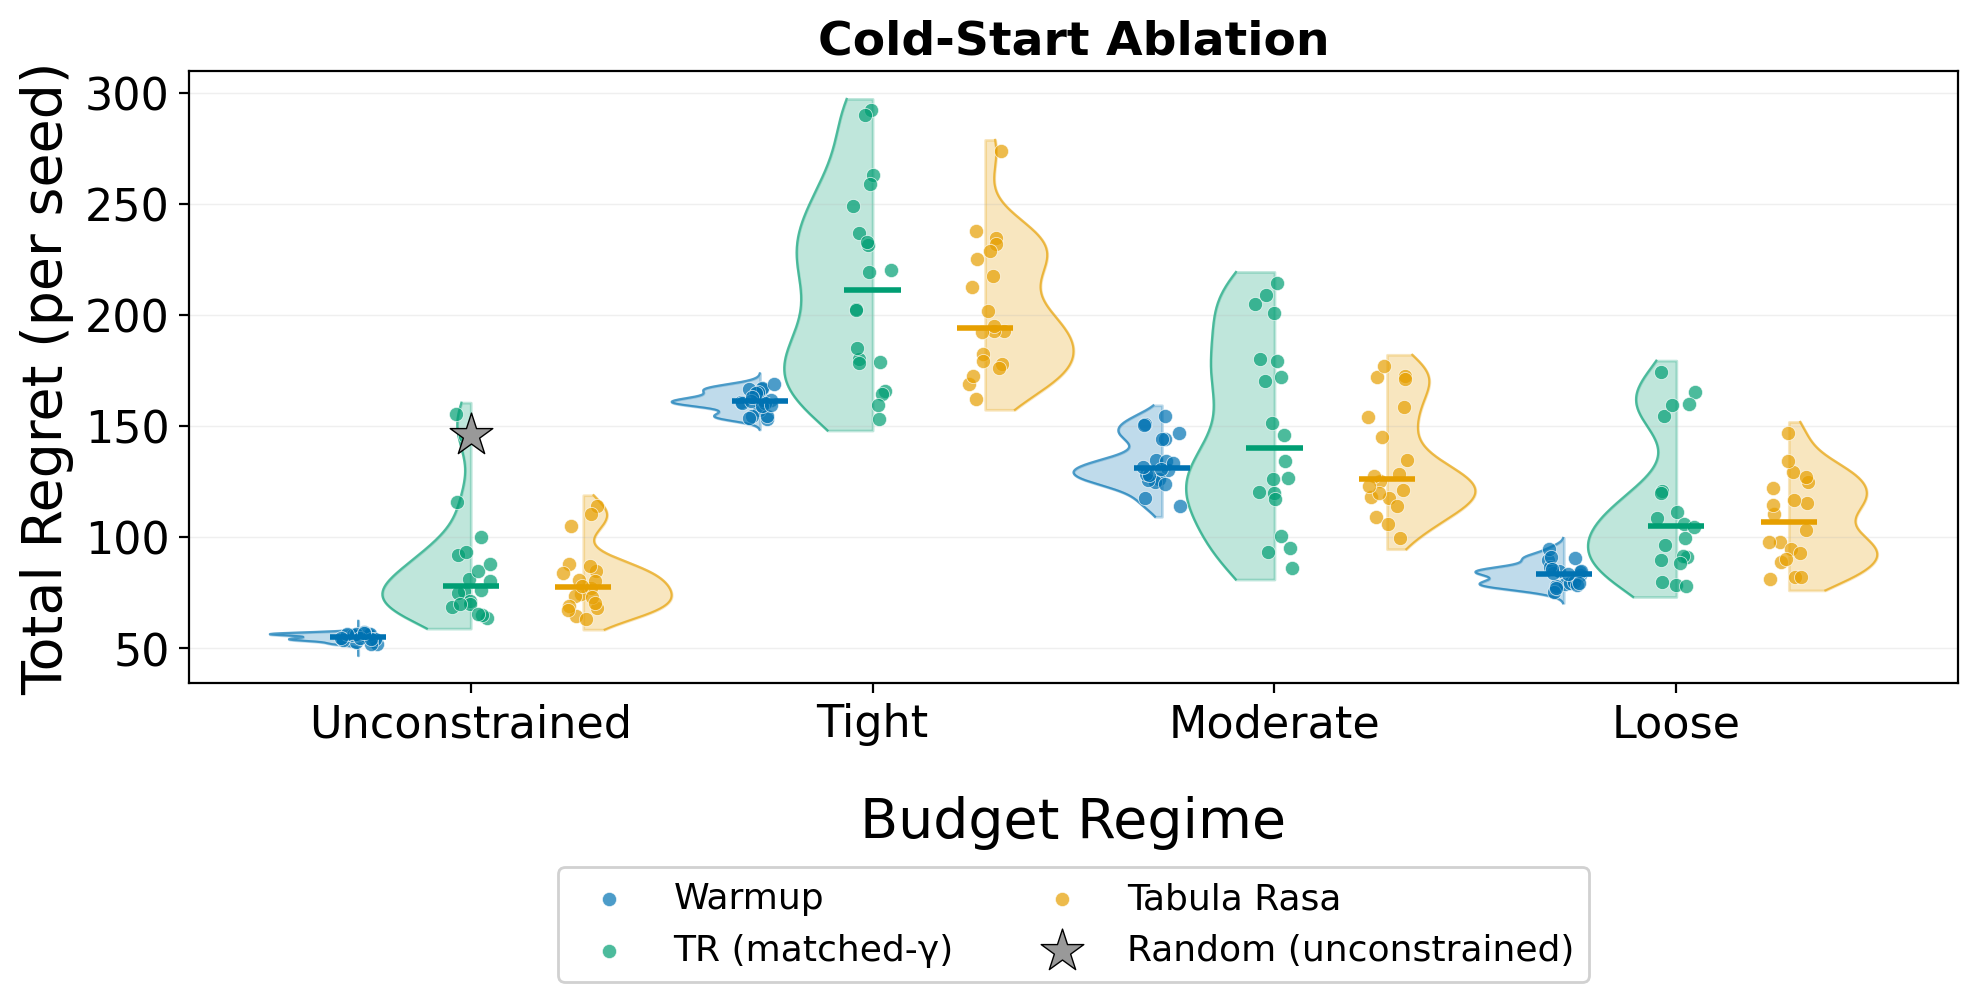
\includegraphics[width=\columnwidth]{../experiments/appendix/warmup_ablation/results/warmup_ablation.png}
\caption{Cold-start ablation on the $K{=}3$ stationary portfolio (20~seeds, held-out test split, $n{=}1{,}824$ prompts). Per-seed cumulative regret distributions compare warmup priors (blue) against Tabula Rasa (orange) and the matched-$\gamma$ cold-start control (green) across four budget regimes. The corresponding Holm-corrected sign-test results and catastrophic-failure counts under the pooled-median threshold are reported in Table~\ref{tab:warmup_ablation_results}. Warmup priors produce tight, unimodal distributions, while cold-start baselines exhibit heavier tails under budget constraints due to the pacer--exploration interaction.}
\label{fig:warmup_ablation}
\end{figure}
